\documentclass{article}

\usepackage{tikz}
\usetikzlibrary{positioning}
\tikzset{every picture/.style={>=latex}}

\begin{document}

\newcommand\mst\mathstrut

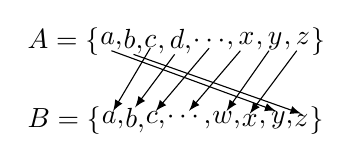
\begin{tikzpicture}[every node/.style={inner sep=0pt},node distance=0pt]
\node[right] (A) at (0,0) {$A=\{\mst$};
\node (a) [right=of A] {$a,\mst$};
\node (b) [right=of a] {$b,\mst$};
\node (c) [right=of b] {$c\mst$};
\node (d) [right=of c] {$,d,\mst$};
\node (cdots) [right=of d] {$\cdots\mst$};
\node (x) [right=of cdots] {$,x\mst$};
\node (y) [right=of x] {$,y\mst$};
\node (z) [right=of y] {$,z\mst$};
\node [right=of z] {$\}\mst$};

\node[right] (B) at (0,-1) {$B=\{\mst$};
\node (a1) [right=of B] {$a,\mst$};
\node (b1) [right=of a1] {$b,\mst$};
\node (c1) [right=of b1] {$c,\mst$};
\node (cdots1) [right=of c1] {$\cdots,\mst$};
\node (w) [right=of cdots1] {$w,\mst$};
\node (x1) [right=of w] {$x\mst$};
\node (y1) [right=of x1] {$,y,\mst$};
\node (z1) [right=of y1] {$z\mst$};
\node [right=of z1] {$\}\mst$};

\draw [->] (a.south) -- (y1.north);
\draw [->] (b.south) -- (z1.north);
\draw [->] (c.south) -- (a1.north);
\draw [->] (d.south) -- (b1.north);
\draw [->] (cdots.south) -- (c1.north);
\draw [->] (x.south) -- (cdots1.north);
\draw [->] (y.south) -- (w.north);
\draw [->] (z.south) -- (x1.north);
\end{tikzpicture}

\end{document}